\section{Initial Experiment Results} \label{sec:exp_results}
\brett{go through this section again, need to fill it out some more}
\nisar{...feels like this part is missing some detail? (e.g. breakdown of subjects, protocol for screening/paying, etc.) not sure, but this seems important for human factors audience...}
Here, we present some preliminary findings in an experiment to meant to investigate whether \xQ{} and \xO{} have effects on user behavior and perception. In order to do this we designed an Amazon Mechanical Turk experiment where human users acted as dispatch supervisors of the unmanned delivery truck described in Sec.~\ref{sec:donut_delivery}. They key hypothesis is that users who are presented with self-confidence metrics will perform better in the dispatch task which will be reflected in a higher score.

\begin{figure}[tbp]
    \centering
    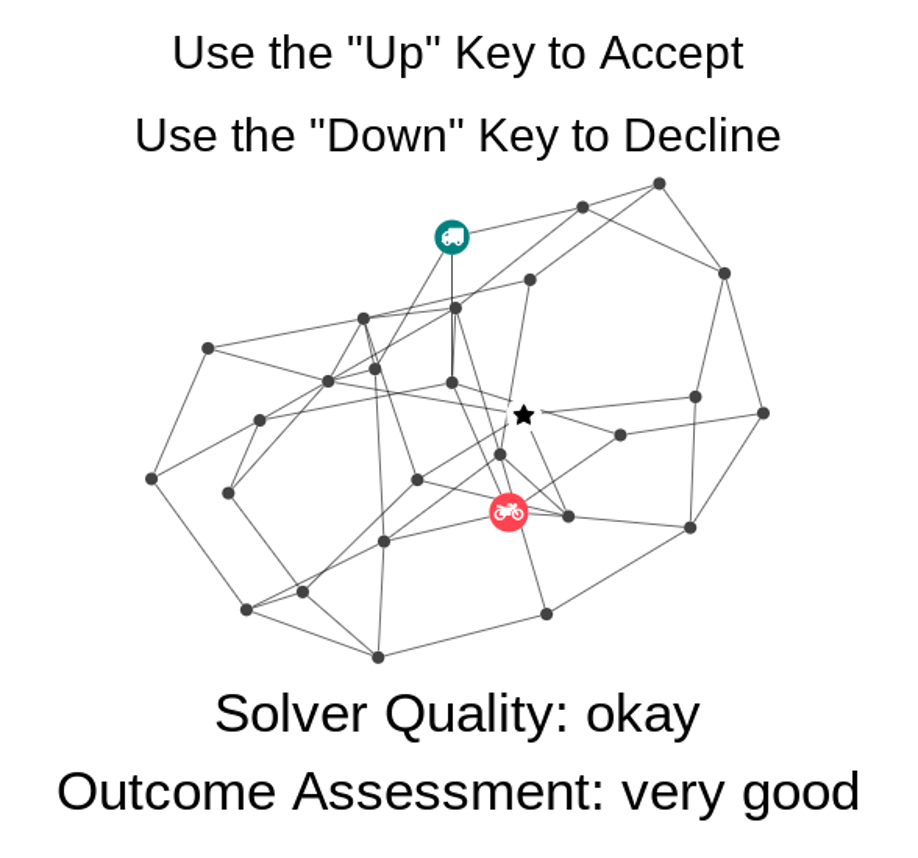
\includegraphics[width=0.45\linewidth]{Figures/experiment_screenshot_Compressed.png}
    \caption{Example screenshot from the Amazon Mechanical Turk experiment.  } 
    \label{fig:experiment_screenshot}
\end{figure}

In Fig.~\ref{fig:total_score} both \xQ{} and \xO{} are displayed, indicating that the user is in condition 4. Other conditions have identical layout but with the values for \xQ{} and/or \xO{} missing according to the experiment design.

The responsibility of each participant was to decide whether the autonomous delivery vehicle should attempt to make a delivery, or decline the delivery. A successful attempt resulted in +1 point, failure in -1 point, and declining a delivery in -1/4 point. After being trained the participants saw a sequence of 43 different delivery scenarios with varying maps. The experiment was a between-subjects design with 4 conditions. The first condition was the control condition where the users only had the map to use to make decisions. In condition 2 users were presented with \xQ{}, and in condition 3 they were shown \xO{}. In condition 4 users were given both \xQ{} and \xO. A screenshot of a typical task is shows in Fig.~\ref{fig:experiment_screenshot}. Based on feedback from a pilot study the numerical values for \xQ{} and \xO{} were subdivided into regions and converted to words such as `very good' or `bad' to help users more easily grasp the scales.

Some preliminary data comparing the difference in cumulative `total score' is shown in Figure~\ref{fig:total_score}. The total number of participants represented here is N=255, with $n=\{63,63,64,65\}$ for conditions 1-4 respectively. Statistically the score for participants from each of conditions 2-4 have a significantly higher mean that of participants from condition 1. This indicates that the participants were able to recognize limitations of the UDT and make better dispatch decisions. Informally it looks like those users in condition 4 performed better than all other conditions, but the significance of that difference still needs to be investigated.

\begin{figure}[tbp]
    \centering
    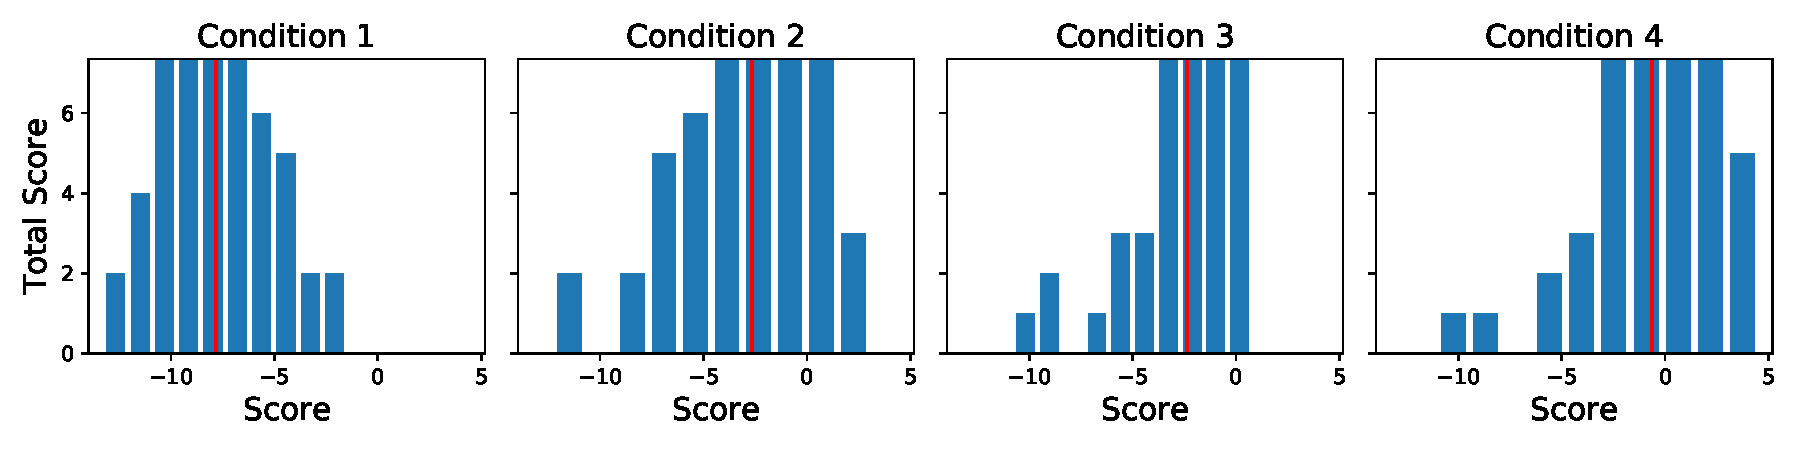
\includegraphics[width=1.0\linewidth]{Figures/total_score.pdf}
    \caption{Histogram of the Total Score from each condition. Red vertical lines denotes the sample mean. \brett{Insert p-values and statistics}}
    \label{fig:total_score}
\end{figure}

At the end of the experiment participants answered survey questions about their perception of the UDT, how much they trusted the system, and how capable they thought it was. Our hypothesis is that the presence of self-confidence metrics would also affect these responses, but this data is still being analyzed.

%
% \begin{table}[]
% \centering
% \caption{Put in some statistics here---p-values}
% \label{tab:results}
% \begin{tabular}{lllll}
 % &  & B & C & D \\ \cline{1-1}
% \hline
% x\_Q & 0.998 & 0.667 & 1.095 & 1.351 \\
% x\_Q & 0.994 & 0.215 & 1.291 & 1.821 \\
% \end{tabular}
% \end{table}
